\documentclass[12pt,a4paper,twoside,openany]{book}
\usepackage{textcomp}
\usepackage[T1]{fontenc}
\usepackage[utf8]{inputenc}
\usepackage[italian]{babel}
\usepackage{pdfpages}
\usepackage{graphicx}
\usepackage{rotating}
\usepackage{listings}
\usepackage{caption}
\usepackage{float}
\usepackage{booktabs}
\usepackage{picture}
\usepackage{multirow}
\usepackage{pifont}
\usepackage[hidelinks]{hyperref}
\usepackage{tikz}
\usetikzlibrary{fit,shapes.geometric}

\providecommand*{\cmark}{\ding{51}}
\providecommand*{\xmark}{\ding{55}}

\newcounter{nodemarkers}
\newcommand\circletext[1]{%
	\tikz[overlay,remember picture] 
	\node (marker-\arabic{nodemarkers}-a) at (0,1.5ex) {};%
	#1%
	\tikz[overlay,remember picture]
	\node (marker-\arabic{nodemarkers}-b) at (0,0){};%
	\tikz[overlay,remember picture,inner sep=2pt]
	\node[draw,ellipse,fit=(marker-\arabic{nodemarkers}-a.center) (marker-\arabic{nodemarkers}-b.center),color=red] {};%
	\stepcounter{nodemarkers}%
}

%codice per mettere logo in sfondo ad ogni pagina
\usepackage{eso-pic}

\AddToShipoutPicture
{
  \put(\LenToUnit{.4\textwidth}, \LenToUnit{.5\textheight}){
\includegraphics{immagini/logo}}%
}

\lstset{basicstyle=\footnotesize\ttfamily\color{black}, language=vhdl, keywordstyle=\color{blue}\bfseries, stringstyle=\color{black}, showstringspaces=false, frame=single, numbers=left, numbersep=5pt, numberstyle=\tiny\color{black}}

\graphicspath{immagini/}
\author{Antonio Riccio - Mat. M63/0605
\and Andrea Scognamiglio - Mat. M63/0598
\and Stefano Sorrentino - Mat. M63/0630}
\title{Zynq GPIO \\ Gruppo 3}

\begin{document}
\frontmatter
\maketitle
\setcounter{page}{1}
\mainmatter
\chapter*{GPIO}
Il progetto consiste  nella realizzazione di un componente GPIO, \textit{General Purpose Input/Output},  dalla descrizione hardware in VHDL fino alla definizione dei relativi driver a diversi livelli di astrazione.

In questo documento verranno illustrati i concetti fondamentali e le decisioni di progetto che hanno portato alla realizzazione degli artefatti finali, per approfondimenti si rimanda alla documentazione interna e al codice sorgente allegati. 

\section*{Descrizione del componente}
La descrizione in VHDL non è molto impegnativa data la natura semplice del componente. Questo è stato descritto mediante un'assegnazione condizionata che ne descrive il comportamento mediante l'utilizzo di una porta \textit{tri-state}. 

La descrizione nel dominio \textit{data flow} del componente  è riportata di seguito:
\begin{lstlisting}[caption={componente GPIO}, label={}, captionpos=b]
entity gpio_pad is
    Port ( pad_out : in STD_LOGIC; 
           pad_en : in STD_LOGIC;  
           pad_in : out STD_LOGIC; 
           pad : inout STD_LOGIC); 
end gpio_pad;

architecture DataFlow of gpio_pad is

begin

pad <= pad_out when pad_en = '1'
       		else 'Z';
pad_in <= pad;

end DataFlow;
\end{lstlisting}

Il segnale di abilitazione \textit{pad\_en} regola la direzione del dato in scrittura, se alto consente la scrittura del dato verso l'esterno, se invece il segnale è basso il componente lavora in sola lettura, dato che la porta \textit{tri-state} è in alta impedenza e l'assegnazione di \textit{pad\_in} è l'unica ad essere abilitata (in realtà è sempre abilitata anche quando il componente lavora in modalità di scrittura).
\clearpage
\subsection*{Interruzioni}
La logica di generazione delle interruzioni è stata descritta in dominio \textit{data flow} per avere un maggior controllo sugli elementi costituenti la circuiteria in modo da garantire efficienza ma anche per garantire un controllo a grana fine delle interruzioni, che si spingesse fino al singolo pin.

Il circuito, il cui schema a blocchi è rappresentato nella \figurename~\ref{gpio_schema_blocchi}, consente il rilevamento della presenza di interruzione solo sul fronte di salita del segnale proveniente dalla fonte interrompente e consente il mascheramento e l'acknowledge delle interruzioni mediante segnali che vanno a pilotare opportunamente gli elementi costituenti.
\begin{figure}[hb]
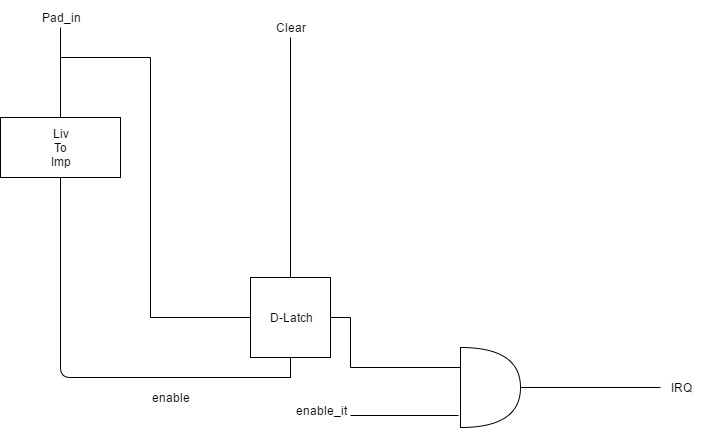
\includegraphics[scale=0.55, keepaspectratio]{immagini/gpio_intgen_schema_blocchi}
\caption{Schema a blocchi}
\label{gpio_schema_blocchi}
\end{figure}

Sostanzialmente il circuito fa uso di un \textit{latch} per mantenere l'informazione circa l'evento di interruzione. L'uscita dato del \textit{latch} corrisponderà al bit di pending dell'interruzione.\\
L'ingresso di \textit{clear} del circuito, che consente di effettuare l'acknowledge dell'interruzione sul pin, è collegato direttamente al segnale di reset asincrono del \textit{latch}, di tipo 1-attivo.\\
Il segnale di IRQ verso il gestore delle interruzioni verrà asserito solo se l'interruzione per quel pin non è stata mascherata attraverso il segnale di \textit{enable}, il quale è messo in \textit{AND} con l'uscita dato del latch. Una porta \textit{OR} può essere messa in uscita alla \textit{AND} nel caso il parallelismo del circuito, quindi il numero di fonti interrompenti, sia maggiore di uno. In tal caso infatti, basterebbe almeno una linea alta di interruzione per generare il segnale IRQ, a meno che le interruzioni per quel pin non risultino mascherate.\\
La logica di rilevamento del fronte del segnale proveniente dalla fonte interrompente è demandato al componente \textit{livelli2impulsi} che non è altro che un piccolo automa a due stati che genera un segnale impulsivo a partire da un segnale a livelli. Questo componente è necessario per consentire al \textit{latch} la memorizzazione dell'informazione riguardante l'avvento di interruzione solo nell'istante in cui si verifica l'evento ed evitare quindi che il \textit{latch} permanga in trasparenza anche quando non sia necessario.
\section*{Driver}
Il driver \textit{standalone} per il dispositivo è costituito da due livelli. Un primo livello, \textit{gpio\_ll}, che fornisce solo funzioni di base per l'accesso diretto ai registri ed un secondo livello, che racchiude il primo e lo arricchisce fornendo ulteriori servizi per il controllo delle interruzioni.

L'introduzione di un secondo livello è nata dalla necessità di riusare il codice già scritto in precedenza per la prima versione del componente, che non aveva il supporto alle interruzioni, e di implementare controlli sui dati forniti in input. Lo sviluppo del secondo livello viene incontro proprio a queste necessità.

Si rimanda alla documentazione interna allegata per ulteriori approfondimenti riguardo le API.

\subsection*{Variante in C++}
Una versione in C++ dello stesso driver \textit{standalone} è stata sviluppata con l'intento di studiarne le differenze rispetto a quello scritto in C.
 
Una differenza che si può subito notare è come il C++ consenta di utilizzare i servizi offerti dal driver senza specificare, ad ogni chiamata di funzione,  la particolare periferica sulla quale agire. 
Questo perché le informazioni riguardanti lo specifico componente sono racchiuse all'interno di un oggetto, sul quale è possibile invocare i metodi della classe a cui appartiene poiché un oggetto rappresenta un'\textit{istanza} di quella classe.

E' possibile definire oggetti anche nel C attraverso il meccanismo delle strutture con l'unica differenza che non esiste la caratteristica di oggetto inteso istanza di una data classe, pertanto questa associazione deve essere necessariamente esplicitata dal programmatore, ovvero specificando l'oggetto particolare ad ogni chiamata di funzione. 

\subsection*{Linux}
Il dispositivo è corredato anche di driver scritti per il kernel Linux. In particolare, sono state sviluppate diverse varianti di driver ognuna delle quali utilizza un servizio diverso del kernel per interfacciarsi con il dispositivo, ovvero attraverso la system call \textit{mmap} ed attraverso  il servizio \textit{Userspace Input/Output} o UIO.

Un'ulteriore versione del driver è stata sviluppata come modulo del kernel. Questa è sicuramente la versione più sofisticata delle soluzioni fin ora citate poiché richiede un'ampia conoscenza delle strutture dati e delle funzioni di basso livello del Linux kernel. Infatti lo sviluppo di questa versione ha richiesto molto più tempo rispetto alle versioni precedentemente enunciate.
Uno degli obiettivi prefissati per lo sviluppo di questo driver è stato quello della \textbf{generalità}: il driver è stato scritto tenendo in mente la necessità di gestire tutte le operazioni possibili sul dispositivo, ovvero operazioni di lettura e di scrittura. 
Altro vincolo fondamentale è stato quello di voler gestire contemporaneamente più dispositivi (funzionanti anche in diverse modalità, ovvero lettura e/o scrittura) e quindi trattare tutti quei problemi di concorrenza che ne sono associati.
La spiegazione nel dettaglio del funzionamento di quest'ultima versione esula dagli scopi di questo documento, pertanto si rimanda al codice sorgente, accuratamente commentato, per approfondimenti riguardanti il significato delle singole istruzioni.
\section*{Sviluppi futuri}
Questa sezione è stata scritta con l'intento di illustrare possibili miglioramenti al progetto che, per motivi di tempo, non stati implementati ma che lo potrebbero essere in versioni future del componente.

Un primo miglioramento consisterebbe nell'ottimizzazione dello spazio di indirizzamento del componente hardware. L'intento sarebbe quello di gestire con un unico indirizzo più registri, accessibili quindi o in sola lettura o in sola scrittura e ridurre in tal modo l'area di memoria necessaria per la gestione del componente.

Un altro miglioramento potrebbe essere quello di rendere l'unità di generazione delle interruzioni configurabile dal punto di vista del tipo di evento interrompente. L'idea è quella di arricchire il componente di generazione delle interruzioni con la possibilità di far decidere all'utilizzatore il tipo di evento sul quale generare richiesta di interruzione, che possa essere rilevare anche fronti di discesa o a livelli del segnale proveniente dalla fonte interrompente.

Dal punto di vista del controllo delle interruzioni, si potrebbe invece pensare di implementare la possibilità di abilitare/disabilitare le interruzioni a livello globale in modo da consentire un controllo più veloce della parte di generazione delle interruzioni.
\end{document}
